\section{2d Web Symbols and Icons}


\begin{figure}
	\centering
	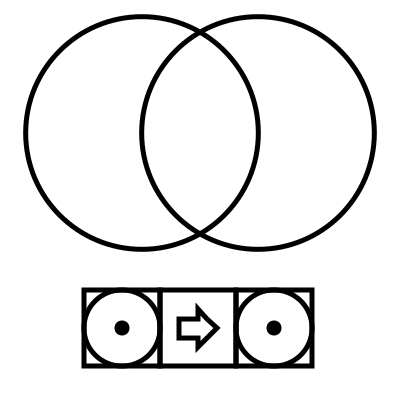
\includegraphics[width=4in]{figures/web2d/vesicapiscis.png}
	\caption[vesicapiscis]
	{The ``hello world'' of geometric programming, the Vesica Piscis.}
\end{figure}


\begin{figure}
	\centering
	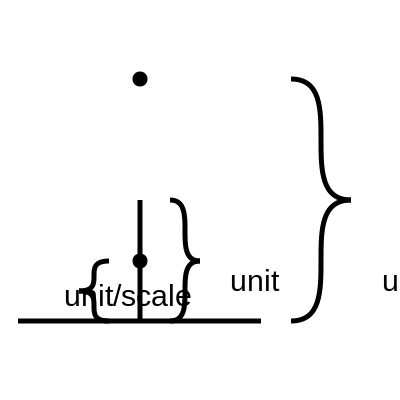
\includegraphics[width=4in]{figures/web2d/cursorscale1.png}
	\caption[cursorscale]
	{Cursor scale.}
\end{figure}
\begin{figure}
	\centering
	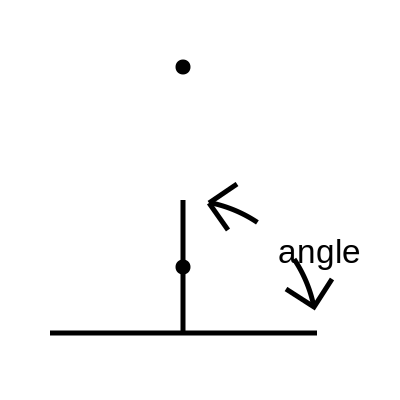
\includegraphics[width=4in]{figures/web2d/cursorangle1.png}
	\caption[cursorangle]
	{Cursor angle.}
\end{figure}
\begin{figure}
	\centering
	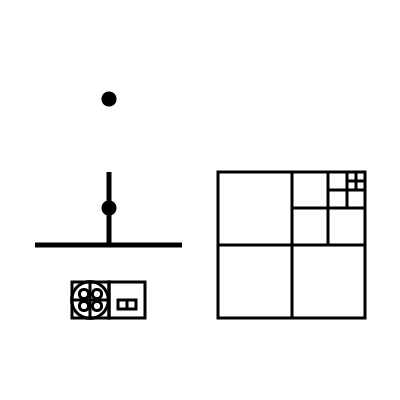
\includegraphics[width=4in]{figures/web2d/cursorsquare.png}
	\caption[cursorsquare]
	{Cursor square.}
\end{figure}
\begin{figure}
	\centering
	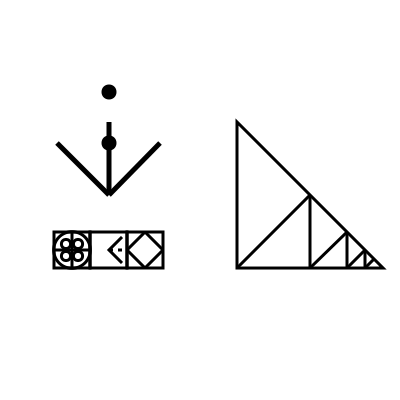
\includegraphics[width=4in]{figures/web2d/cursorroot2.png}
	\caption[cursorroot2]
	{Cursor root2.}
\end{figure}
\begin{figure}
	\centering
	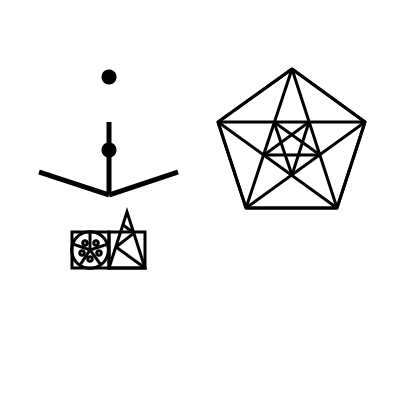
\includegraphics[width=4in]{figures/web2d/cursorgolden.png}
	\caption[cursorgolden]
	{Cursor golden ratio.}
\end{figure}
\begin{figure}
	\centering
	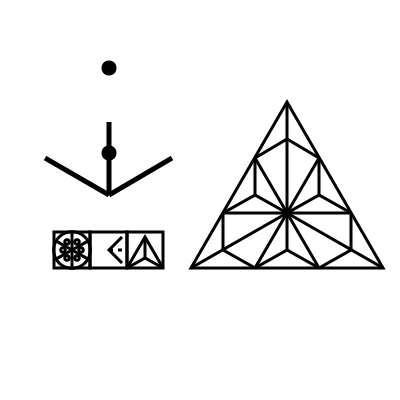
\includegraphics[width=4in]{figures/web2d/cursorroot3.png}
	\caption[cursorroot3]
	{Cursor root 3.}
\end{figure}
\begin{figure}
	\centering
	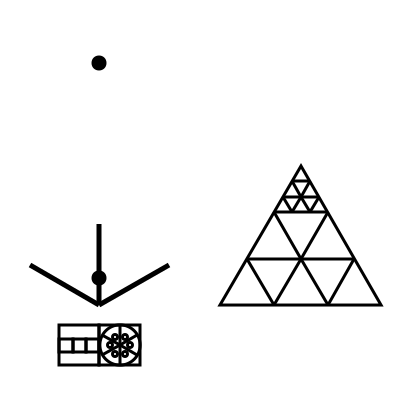
\includegraphics[width=4in]{figures/web2d/cursor3.png}
	\caption[cursor3]
	{Cursor 3.}
\end{figure}
\begin{figure}
	\centering
	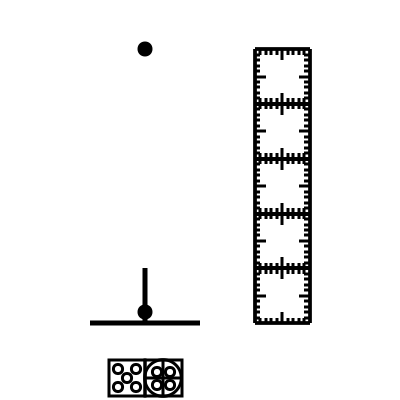
\includegraphics[width=4in]{figures/web2d/cursor5.png}
	\caption[cursor5]
	{Cursor 5.}
\end{figure}





\begin{itemize}
\tightlist
\item
hello world vesica piscis
\item
symbols, how they work with hypercube, 
\item
editing, cursor, keyboards, control panels, modes
\item
symmetries and scales, different methods of geometron(AG)
\item
cursor,movements, basic constructions(segment, circle, arc, dot)
\item
layers, colors, lines, style json, working with styles, transparency in hex colors, finding colors
\item
bezier curves
\item
paths
\item
character stack
\item
fonts
\item
flags
\item
tracing symbols from images
\item
editing the hypercube and shape table, sharing them, import and export of hypercube, sharing of bytecode
\item
canvas,svg/png/base64 workflow, laser cut shapes production, practical graphics for manuscripts and web, iconsymbols, usage in jupyter notebooks, how the JSON embeds in the SVG, how the symbol feed works, how the setup of JSON works,
\item
control panels, softkey interfaces, writing geometron apps, how to replicate in other systems from scratch
\item
examples of using the GVM in JS, documentation of geometron.js, how to use
\end{itemize}